\documentclass[14pt]{beamer}

\usepackage{listings}
\lstloadlanguages{python}

\usepackage{color}
\usepackage{tikz}


\mode<presentation>
{
\usetheme{AlpesLasers}
\setbeamercovered{transparent}
  %\setbeamertemplate{footline}[frame number] 
  %\setbeamertemplate{navigation symbols}{ 
  %\hskip 0.3cm
  %\insertframenumber / \inserttotalframenumber  % <<< frame #
  %\insertpagenumber / \insertpresentationendpage % <<< page #
%} 
}

% font definitions, try \usepackage{ae} instead of the following
% three lines if you don't like this look
\usepackage{mathptmx}
\usepackage[scaled=.90]{helvet}
\usepackage{courier}
\usepackage[T1]{fontenc}
\usepackage[english]{babel}
\usepackage[latin1]{inputenc}
\title{The Alpes Lasers use case}
\subtitle{ALDIRAC}
\author{St\'ephane Poss}
\date{\today}
% This is only inserted into the PDF information catalog. Can be left
% out.
\subject{ALDIRAC}


\begin{document}
\begin{frame}[plain]
\titlepage
\end{frame}

\section{Introduction}
\begin{frame}
\frametitle{Outline}
\begin{itemize}
\setlength{\itemindent}{-1.2em}
\item Context
\item Use case
\item Work model
\item Application workflow
\item User Interface
\item Dedicated system
\end{itemize}
\end{frame}

\section{Alpes Lasers use case}
\begin{frame}
\frametitle{Who is Alpes Lasers?}
\begin{itemize}
\setlength{\itemindent}{-1.2em}
\item Specialized in Quantum Cascade Lasers (QCL) in mid infrared
\item In Neuch\^atel, Switzerland
\item 20 people
\item \alert{World leader}: many experts of the field work here
\item Many different types of clients, from Uni to private sector
\item Mostly research and development activities
\end{itemize}
\end{frame}
%\begin{frame}
%\frametitle{Who is Alpes Lasers?}
%\begin{itemize}
%\end{itemize}
%\end{frame}
{
\usebackgroundtemplate{
\includegraphics[width=\paperwidth]{clients}}
\begin{frame}[plain]
~
\end{frame}
}
\subsection{QCLs ?}
\begin{frame}
\frametitle{What are QCLs?}
\begin{columns}[c]
\column{0.5\textwidth}
\centering
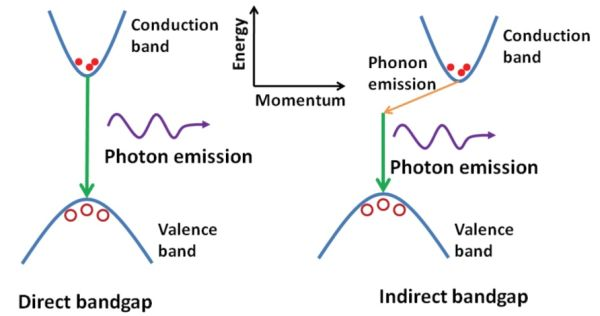
\includegraphics[width=1.2\textwidth]{image1.jpg}\\
Interband
\column{0.5\textwidth}
\centering
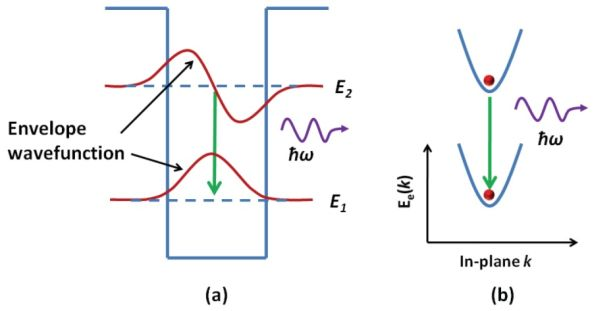
\includegraphics[width=1.2\textwidth]{image18.jpg}\\
\alert{Intersubband} (QCLs)
\end{columns}
\begin{columns}[c]
\column{0.7\textwidth}
One electron yields $>1$ photon\\
Possible to \alert{tune the wavelength}, operate at \alert{room temperature}!
\column{0.6\textwidth}
\centering
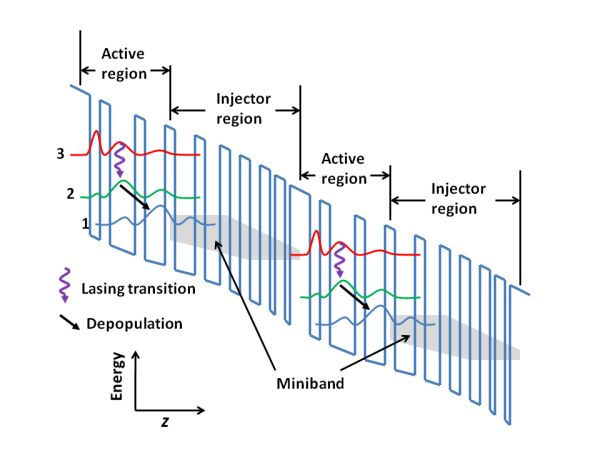
\includegraphics[width=1.1\textwidth]{image21.jpg}
\end{columns}
\end{frame}

\begin{frame}
\frametitle{The optical domains}
\centering
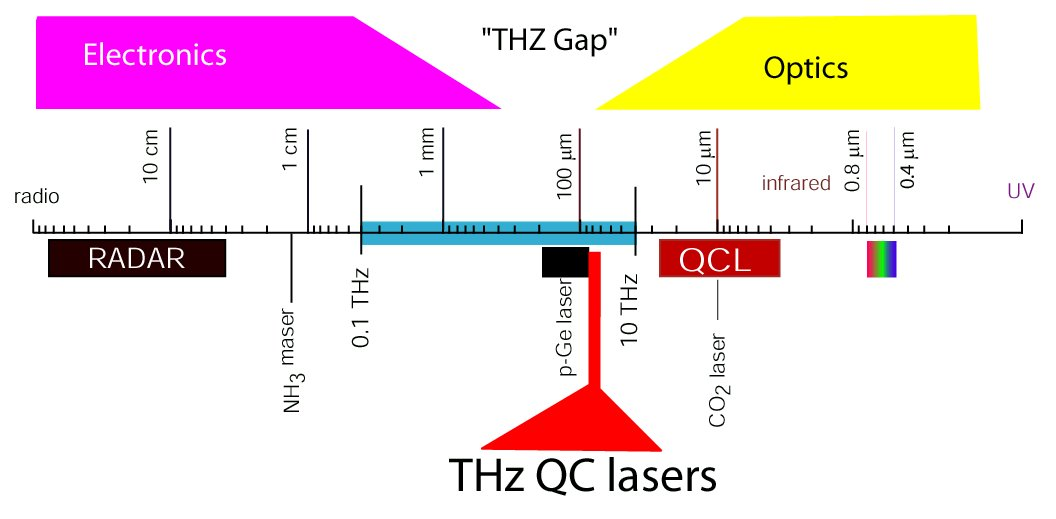
\includegraphics[width=0.8\paperwidth]{wavelengths.png}\\
Obtaining THz emission usually done using FEL

\end{frame}

\begin{frame}
\frametitle{What for?}
\begin{columns}[c]
\column{0.49\textwidth}
Spectroscopy:
\begin{itemize}
\item Trace gas detection
\item Remote sensing
\item Environmental monitoring
\item Quality analysis
\end{itemize}
\column{0.49\textwidth}
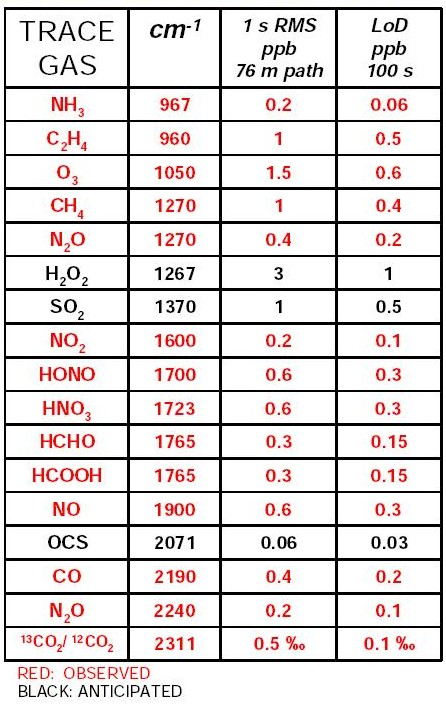
\includegraphics[width=4cm]{spectro.png}
\end{columns}
\alert{Same material system} gives access to \alert{wide range of wavelengths}, \alert{small device} size compared to traditional devices
\end{frame}

\subsection{Why DIRAC?}
\begin{frame}
\frametitle{Why DIRAC? (1)}
\begin{itemize}
\setlength{\itemindent}{-1.2em}
\item QCL tech. is recent, \alert{only 20 years old}
\item No widely established tools
\item \alert{Very hard to build devices}, no complete theoretical models to predict a structure's behavior.
\end{itemize}
\end{frame}

\begin{frame}
\frametitle{Why DIRAC? (2)}
\begin{itemize}
\setlength{\itemindent}{-1.2em}
\item Some software exist (in-house) to predict some of the devices' behavior, need validation against built structures. {\color{blue}Intellectual Property} is involved.
\item Use of Open Source software dominates
\item Do not want to spend time reinventing the wheel and DIRAC seems complete.
\item Can have an expert in house (S.~Poss)
\end{itemize}
\alert{It's a reasonnable, attractive solution}
\end{frame}


\section{Work Model}
\begin{frame}
\frametitle{Our work model}
\begin{itemize}
\setlength{\itemindent}{-1.2em}
\item Do not have a local CE, use \alert{Amazon EC2 with VMDIRAC}
\item {\color{blue}No Storage Element}, need to be careful with Output Data
\item Deal with the {\color{blue}Intellectual Property}
\item Define and implement \alert{dedicated system} to interact with the in-house database (PSQL): SimuDB
\end{itemize}
\end{frame}

\subsection{Cloud running}
\begin{frame}
\frametitle{Amazon EC2}
\begin{itemize}
\setlength{\itemindent}{-1.2em}
\item {\color{blue}No contextualization} but 2 types of machines pre-installed/configured:
\begin{itemize}
\item[Small] 1 core machine for test jobs
\item[Large] Many core machines: Utility to start as many JobAgents as we want
\end{itemize}
\item EC2 provides 32 core machines for \$1.9/hour, could run \alert{up to 640 jobs concurrently} (20 machines)
\item Security group: dedicated ip/ports only
\end{itemize}
\end{frame}

\subsection{Architecture}
\begin{frame}
\frametitle{Available resources in our office}
\begin{itemize}
\setlength{\itemindent}{-1.2em}
\item One central DIRAC server hosted on VM \\ 4 cores, 8GB RAM
\item SSHBatchCE configured and used for tests (2 hosts, 4 cores)
\item 20Mbps download / 2Mbps upload link
\end{itemize}
\alert{Deal with the existing resources}
\end{frame}

\subsection{Software Management}
\begin{frame}
\frametitle{Software Management}
\alert{Account for IP}: strict access control
\begin{itemize}
\setlength{\itemindent}{-1.2em}
\item Software only hosted in our machines
\item Packaging done using our tools, based on python packaging tools (i.e. \emph{pip})
\item Use dependency description (\`a la ILCDIRAC) to resolve all/only soft. bits needed for a job
\item Use \texttt{rsync+ssh} to collect only software differences: reduced software transfer footprint
\end{itemize}
{\color{blue} CVMFS could be an alternative}, if needed.
\end{frame}


\section{Application worklfow}
\begin{frame}
\frametitle{Application workflow}
\centering
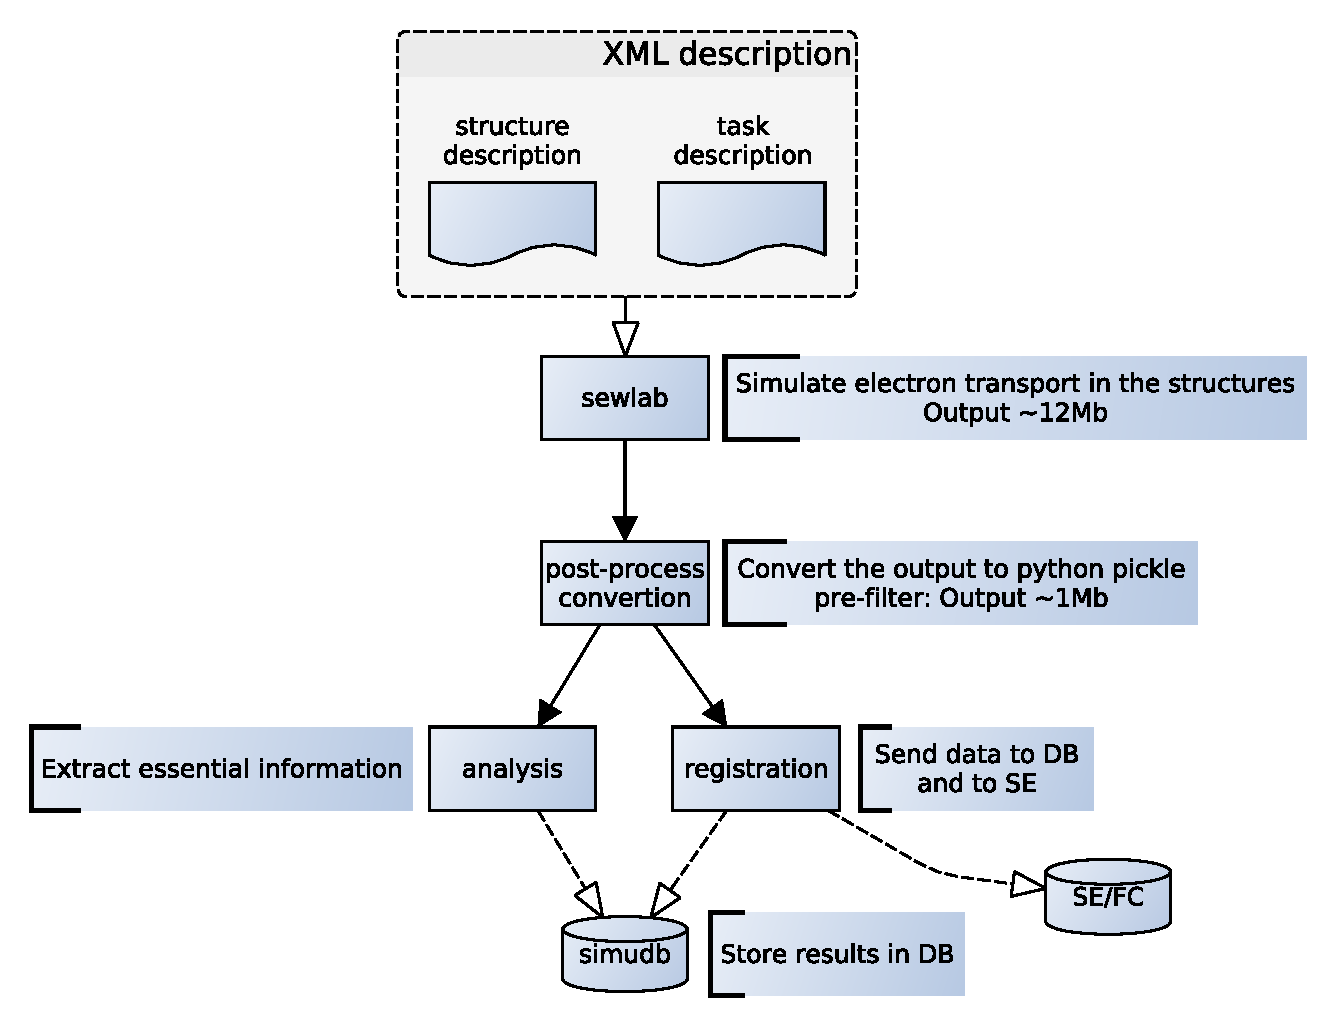
\includegraphics[width=\textwidth]{sewlabworkflow}
\end{frame}

\section{User Interface}
\begin{frame}
\frametitle{User Interface}
Based on ILCDIRAC:
\begin{itemize}
\setlength{\itemindent}{-1.2em}
\item Uses DIRAC's \emph{Workflow}
\item Decoupling of Applications and Jobs
\item Uses \alert{Template Method} pattern
\item Took an afternoon to get the UI working
\item Adding a new application is fast
\end{itemize}
\end{frame}

\section{SimuDB}
\begin{frame}
\frametitle{Dedicated system: SimuDB}
{\color{blue}Decouple ALDIRAC from Alpes Lasers' data source} (PostgreSQL DB)
\begin{itemize}
\setlength{\itemindent}{-1.2em}
\item Tasks created in central DB by {\color{blue}external client}
\item Submitted by \alert{dedicated agent} 
\item Tasks' statuses reported by jobs through \alert{dedicated service}
\item \alert{Results inserted in DB directly} by job through service
\end{itemize}
Advantage: loose coupling, ease of change.
\end{frame}

\begin{frame}
%\frametitle{SimuDB}
\vskip -1cm
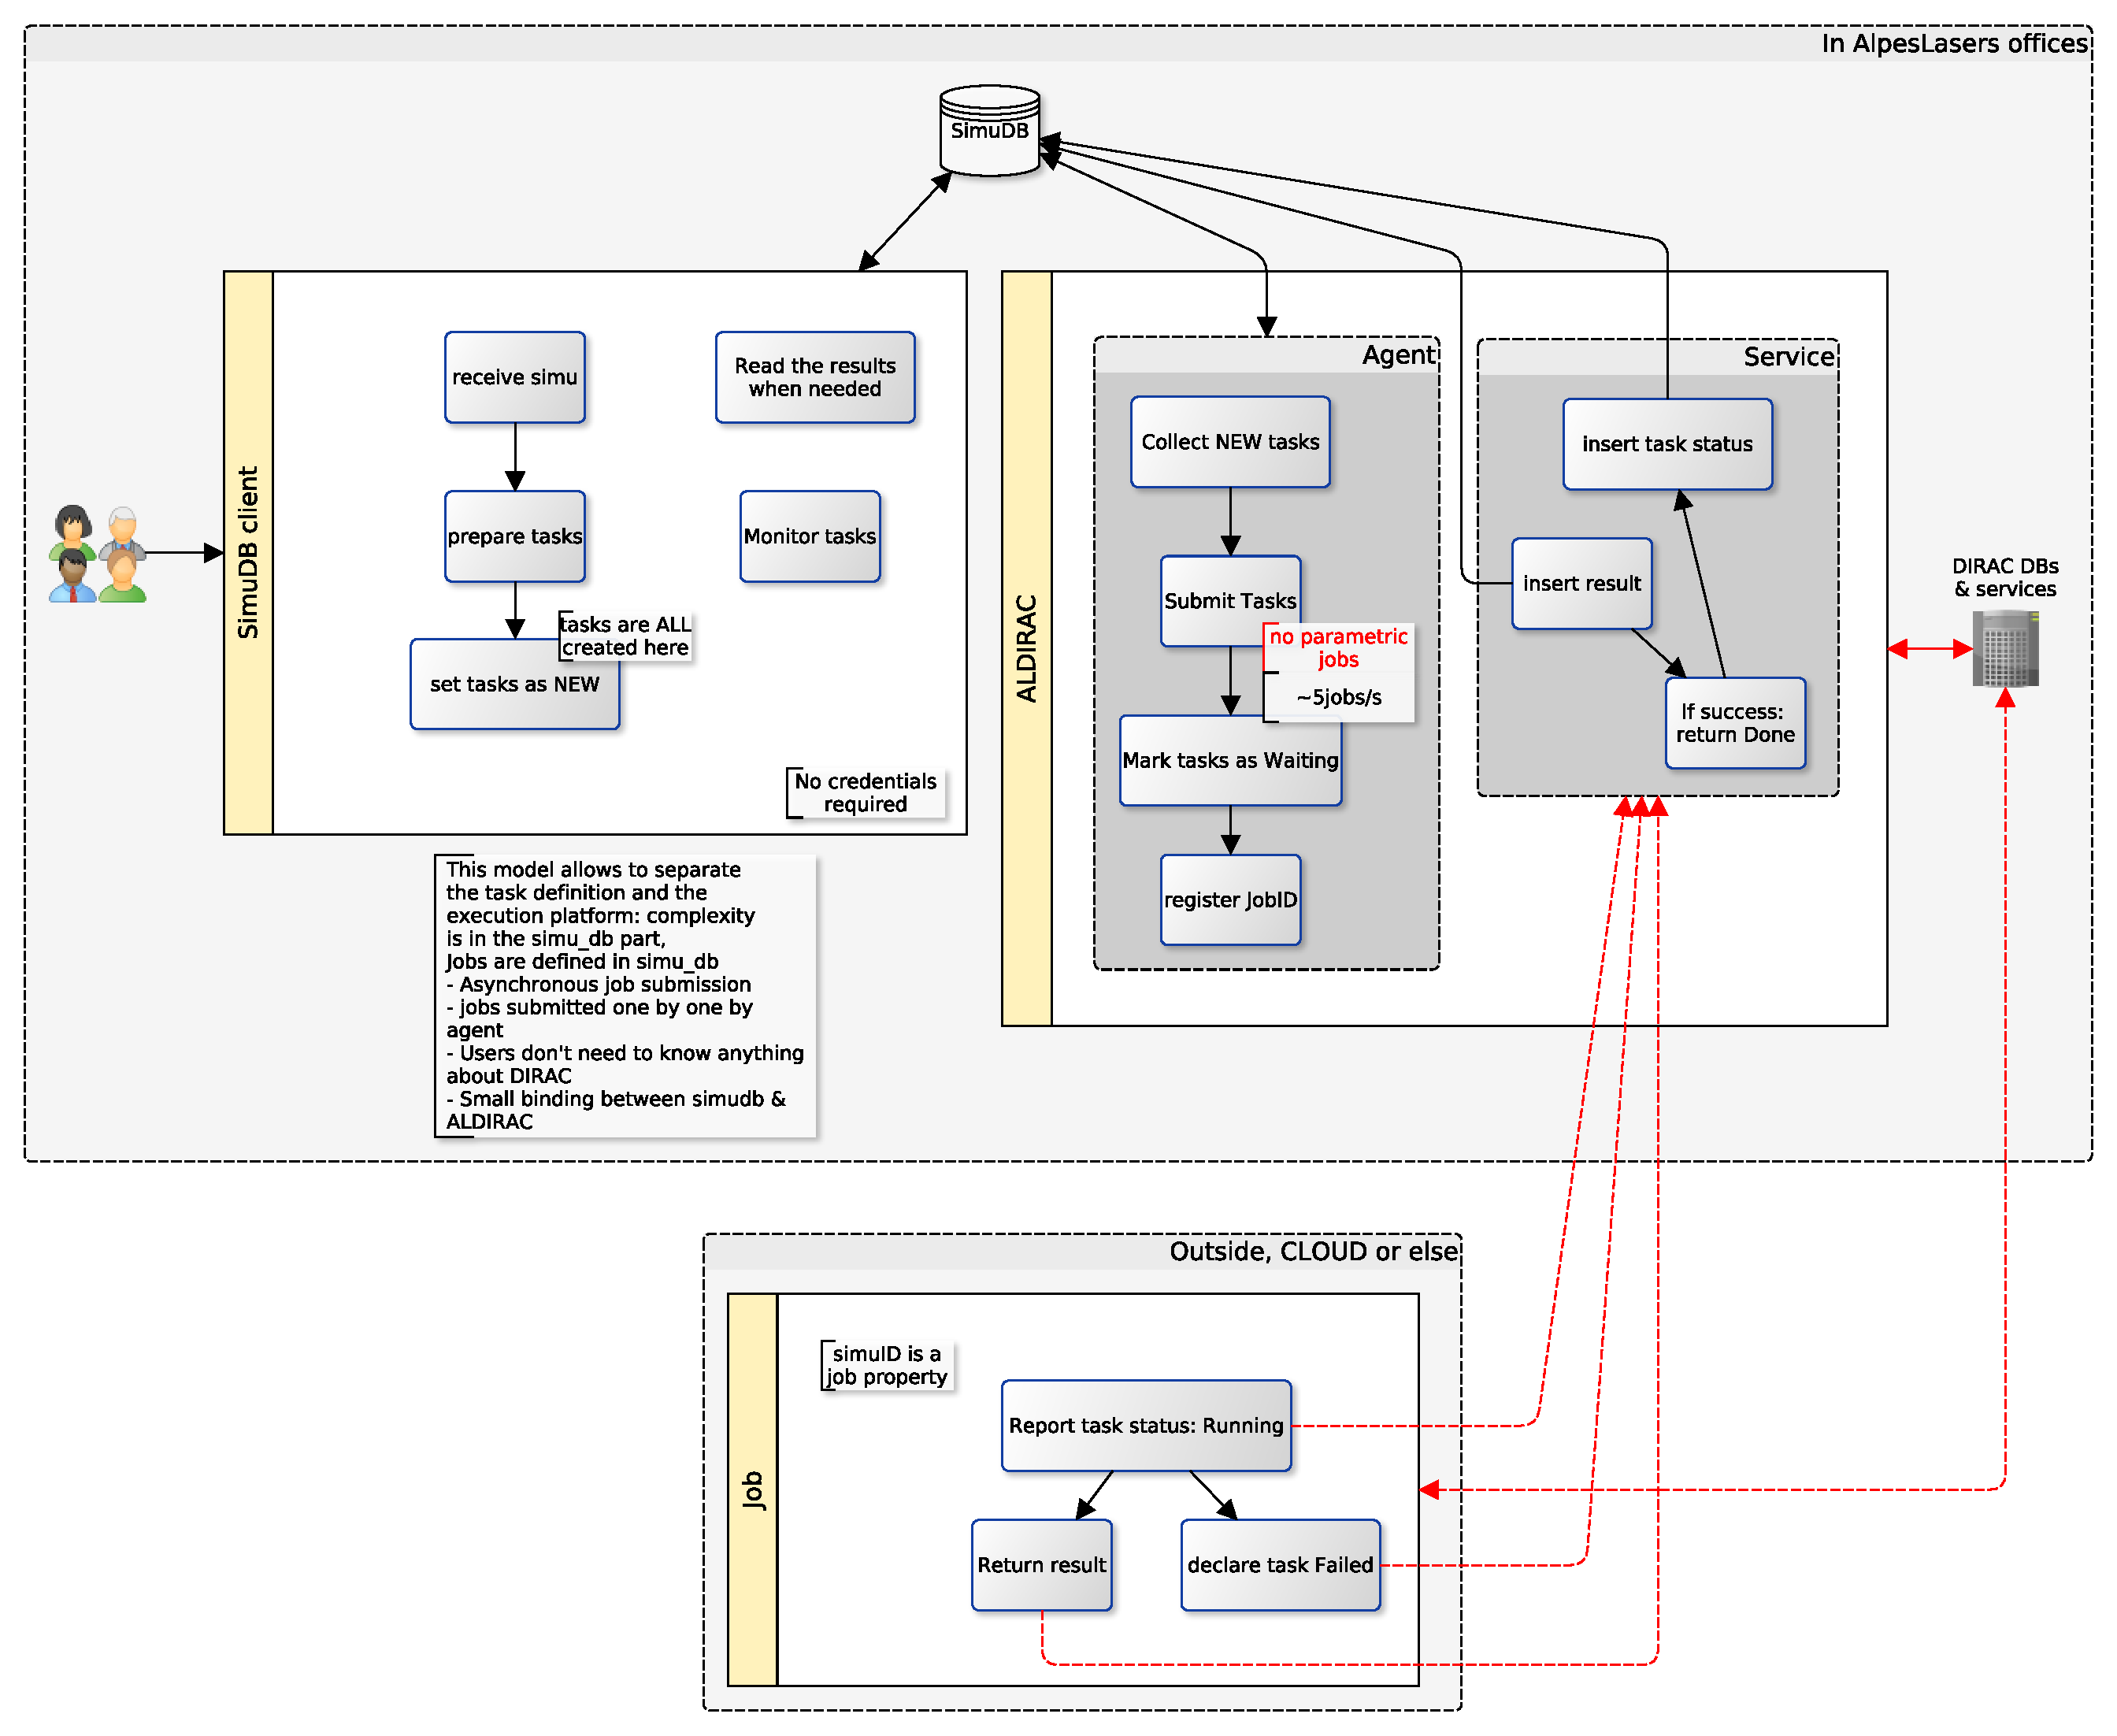
\includegraphics[height=8.2cm]{dirac_arch}
\end{frame}

\section{Prospects}
\begin{frame}
\frametitle{Conclusions and Prospects}
Conclusions:
\begin{itemize}
\item Ran successfully few thousand jobs
\end{itemize}
Prospects:
\begin{itemize}
\item Simulate all existing devices
\item Compare results with measured values
\item Determine quality of simulation tools
\item Add more tools to ALDIRAC
\item Produce a web front end to our workflows to allow clients to interact
\end{itemize}
\end{frame}

%{
%\usebackgroundtemplate{\includegraphics[width=\paperwidth]{cyborg.jpg}}
%\setbeamertemplate{headline}{\includegraphics[width=\paperwidth]{cyborg.jpg}}
%\begin{frame}
%\vspace{6.cm}Thanks to Samuele, Romain, Tobias, \\Antoine, for useful input. More discussions \\will be needed!
%\end{frame}
%}

\end{document}
